
\section{Objectives}
By the end of this laboratory experiment, students are expected to learn how to 

\begin{itemize}

\item model a DC motor, and 
  
\item measure the  speed of a DC motor using a rotary encoder. 
   
\end{itemize}

\section{Parts}
\label{sec:partsDC-MotorModeling}
The following parts are required to conduct this laboratory experiment. %
%
\begin{enumerate}
% \item Breadboard,
\item One 1N4148 diode 
\item $30~[\volt]$ HP 6215 power supply
\item One Pittman DC motor kit
\end{enumerate}

\section{Introduction}
\label{sec:introduction}
This experiment explores the use of a direct current (DC) motor, which is an  electromechanical device that converts DC electrical energy  into mechanical energy.  The motor that will be used in this experiment is the GM8224D201-R-2 Pittman DC motor shown in Figure~\ref{fig:pittmanDC-MotorKit}.  The electrical voltage (DC) applied to the terminals of the motor creates a rotational motion of the motor shaft. The rotational speed of the motor shaft can be controlled by the voltage applied to the motor terminals (red/black wires are connected to the motor's \emph{+ -} terminals (see motor kit shown in Figure~\ref{fig:pittmanDC-MotorKit})). %
%
\begin{figure}
  \centering
  \begin{circuitikz}[american voltages]
    \node[inner sep=0pt]{\includegraphics[width=0.6\textwidth,height=0.3\textheight]{figs/img/pittmanDC-MotorKit}};
    \draw[thick]
    (0*\smgrid,-3.8*\smgrid) |- (-2*\smgrid,-6*\smgrid) -- (-2*\smgrid,-8*\smgrid) to[V,v>=~,l_=$V_a$,fill=green!50] (\smgrid,-8*\smgrid) -- (\smgrid,-3.8*\smgrid);
    
    % Supply to the encoder
    \draw[thick]
    (2.25*\smgrid,-4.35*\smgrid) -- (2.25*\smgrid,-8*\smgrid);
    \draw[thick]
    (2.25*\smgrid,-8*\smgrid) to[V, invert,l_=$V_E$,fill=green!50] (6*\smgrid,-8*\smgrid);%
    %(2.25*\smgrid,-7.5*\smgrid) to[full diode, l_=1N4004 diode] (6*\smgrid,-7.5*\smgrid);
    \draw[thick]
    (6*\smgrid,-8*\smgrid)  to[empty diode, l_=1N4148 diode,fill=blue!50]  (6*\smgrid,-4.35*\smgrid);
    \draw[very thick,<-]
    (3.4*\smgrid,-0.25*\smgrid) to  (11*\smgrid,-0.25*\smgrid)node[right]{Encoder output channel~1};
    \draw[very thick,<-]
    (5*\smgrid,-1*\smgrid) to  (11*\smgrid,-1*\smgrid)node[right]{Encoder output channel~2};    
  \end{circuitikz}
 % \includegraphics[width=0.6\textwidth,height=0.3\textheight]{figs/img/pittmanDC-MotorKit}
  \caption{The Pittman DC motor kit used for the experiment.}
  \label{fig:pittmanDC-MotorKit}
\end{figure}
%
The DC motor kit used in this experiment is equipped with a rotational position sensor (optical rotary encoder), which generates $500$ pulses per revolution [see the label 500 CPR (counts per revolution) on the DC motor kit, which indicates the resolution of the encoder]. The optical rotary encoder mounted in the DC motor kit shown in Figure~\ref{fig:pittmanDC-MotorKit} is electrically isolated from the motor. Therefore, a separate power supply is required for the rotary encoder to operate. The red/black/blue/yellow wires are connected to the rotary encoder, where the red/black wires are used to supply  exactly $5$~[\volt] to the encoder. %
%
\begin{mdframed}[roundcorner=10pt,backgroundcolor=yellow!50]
  {\bf WARNING: The encoder will be damaged if its input voltage (\textit{i.e.,}~$V_{cc}$) exceeds $5$~[\volt] or if the polarity of the input voltage is reversed. Therefore, a diode is required to be connected in series with the supply voltage $V_E$  and the Vcc terminal of the encoder as shown Figure~\ref{fig:pittmanDC-MotorKit}.} 
\end{mdframed}
%
The blue/yellow wires are connected to the two channels of the encoder which are used to measure the rotational speed of the motor shaft.  

\section{Modeling Brushed DC Motor}
\label{sec:motorModeling}
This section briefly illustrates  how to find the transient response (\textit{i.e.,~}rotational speed)  of a motor shaft if it is connected to a gear with the internal rotating part  (\textit{i.e.,~}armature) of the motor. The schematic diagram (including an equivalent electric circuit) of a DC motor is shown in Figure~\ref{fig:DC-MotorSchematic}. Figure~\ref{fig:DC-MotorBD} shows the block diagram of a DC motor, where $V_a(s)$ and $\omega(s)$ are the Laplace transformations of the motor applied voltage $V_a(t)$ and its rotational speed $\omega(t),$ respectively,  for time $t\ge 0.$ The motor field can be excited with a field voltage $V_f,$ which is connected to a field resistance $R_f$ and inductance $L_f.$ The current flowing through the field circuit is $I_f.$ Note that the field circuit is not needed for the permanent magnet motors to be used in this laboratory experiment. %    
%
\begin{figure}
  \centering
  \subfigure[][]{
    \label{fig:DC-MotorSchematic}
    \begin{circuitikz}[scale=1.0,american voltages]
      \usetikzlibrary{patterns}
      \draw
      (0,0) to[short,o-](8*\smgrid,0) to[Telmech=M,n=motor,fill=red!50] ++(0,4*\smgrid);
      \draw[thick,->>]
      (motor.right) -- ++(1.5*\smgrid,0)node[midway,above]{$\omega$};
      \draw[pattern=dots]
      (10*\smgrid,2*\smgrid) ellipse (0.1 and 0.2);
      \draw
      (10*\smgrid,2*\smgrid +0.2) --  (12*\smgrid,2*\smgrid +0.2);
      \draw[ultra thick]
      (10*\smgrid,2*\smgrid -0.2) --  (12*\smgrid,2*\smgrid -0.2)node[midway,below]{\tiny{Mechanical ground}};
      \draw[latex-]
      (12*\smgrid,2*\smgrid -0.2) --  (13*\smgrid,2*\smgrid -0.2)node[right]{$B$};      
      \draw
      (12*\smgrid,1.6*\smgrid) arc (-30:30:0.4);
      \node at (11*\smgrid,2*\smgrid) {$J_m$};
      \draw
      (0,4*\smgrid) to[R,l^=$R_a$,i>=$I_a$,o-] ++(4*\smgrid,0) to [L,l^=$L_a$]++(4*\smgrid,0);
      \draw
      (0,0) to[open,v<=$V_a$] ++(0,4*\smgrid);
      \node at(6.5*\smgrid,2*\smgrid){$V_b$};
      \node at(7*\smgrid,3*\smgrid){$+$};
      \node at(7*\smgrid,1*\smgrid){$-$};

      % Draw fixed field
      \draw
      (12*\smgrid,4*\smgrid)  to[L,l^=$L_f$] (8*\smgrid,5*\smgrid) to[R,l^=$R_f$,i<=$I_f$,-o] (10*\smgrid,8*\smgrid);
      \draw
      (12*\smgrid,4*\smgrid) to[short,-o] (14*\smgrid,7*\smgrid);
      \draw
      (14*\smgrid,7*\smgrid) to[open,v<=$V_f$](10*\smgrid,8*\smgrid);
      \node at (10*\smgrid,5.25*\smgrid) {\emph{Fixed field}};
    \end{circuitikz}
    
  }
  \subfigure[][]{
    \label{fig:DC-MotorBD}
    \begin{circuitikz}[american voltages]
      \draw[-latex]
      (0,0)node[left]{$V_a(s)$} -- (\smgrid,0);
      \draw[fill=lightgray]
      (\smgrid,-\smgrid) rectangle (4*\smgrid,\smgrid);
      \node at(2.5*\smgrid,0){$G_M(s)$};
      \draw[-latex]
      (4*\smgrid,0)-- (5*\smgrid,0) node[right]{$\omega(s)$};
      
    \end{circuitikz}
    }  
  \caption{DC motor~\subref{fig:DC-MotorSchematic} schematic diagram~and~\subref{fig:DC-MotorBD} block diagram.}
  \label{fig:DC-Motor}
\end{figure}
%
The motor parameters that will be used in this laboratory experiment are described in Table~\ref{tab:DC-MotorParameters}. %
%
\begin{table}
  \centering
  \caption{DC motor parameters.}
  \label{tab:DC-MotorParameters}  
  \begin{tabular}{c|l|l}
    \toprule
    Symbol & Description & Unit\\
    \toprule
    $B$&Viscous damping coefficient&$[\si{\newton\cdot\meter\per(\radian\per\second)}]$\\
    $I_a$&Armature current &$[\si{\ampere}]$\\
    $K_E$&Back-emf constant &$[\si{\volt\per(\radian\per\second)}]$\\
    $K_T$&Motor torque constant &$[\si{\newton\meter\per\ampere}]$\\        
    $J_m$&Motor shaft's moment of inertia&$[\si{\kilogram\meter}^2]$\\
    $J_T$& Sum of mass moments of inertia&$[\si{\kilogram\meter}^2]$\\    
    $L_a$&Armature inductance &$[\si{\henry}]$\\
    $R_a$&Armature resistance &$[\si{\ohm}]$\\   
    $T_g$&Motor generated torque &$[\si{\newton\meter}]$\\
    $T_L$&Load torque &$[\si{\newton\meter}]$\\        
    $T_D$&Viscous and friction torque &$[\si{\newton\meter}]$\\    
    $T_f$&Constant coulomb friction torque &$[\si{\newton\meter}]$\\    
    $T_{\mathrm{cf}}$&Coulomb friction torque &$[\si{\newton\meter}]$\\
    $T_{\mathrm{sf}}$&Static friction torque &$[\si{\newton\meter}]$\\
    $T_{\mathrm{gr}}$&Gravity torque &$[\si{\newton\meter}]$\\                
    $V_a$&Motor's applied armature voltage &$[\si{\volt}]$\\
    $V_b$&Motor's back-emf voltage &$[\si{\volt}]$\\
    $\omega$&Motor's rotational speed &$[\si{\radian\per\second}]$\\
    \bottomrule
  \end{tabular}
\end{table}
%
The electric equation of a permanent mangment DC motor are: %
%
\begin{subequations}
  \label{eq:electricModel}
  \begin{align}
    \label{eq:motorElectrical}
    V_a(t) & = I_aR_a + L_a\frac{\mathrm{d}I_a(t)}{\mathrm{dt}} + V_b(t),~~\mathrm{where}\\
    \label{eq:Vb}
    V_b(t) & = K_E\omega(t).
\end{align}  
\end{subequations}
%
Taking the Laplace transformations of Equations~\eqref{eq:motorElectrical}~and~\eqref{eq:Vb}, and then simplifying yields: %
%
\begin{align}
  \label{eq:Ias}
  I_a(s) =   \frac{1}{L_as +R_a}\left[V_a(s) - K_E\omega(s)\right],
\end{align}
%
which is described using the block diagram as shown in Figure~\ref{fig:dcMotorElectric}. %
%
\begin{figure}
  \centering
  \subfigure[][]{
    \label{fig:dcMotorElectric}
    \fcolorbox{white}{gray!15}{
  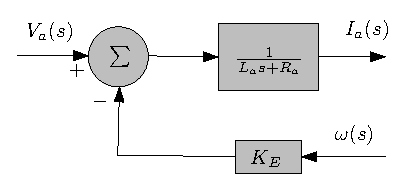
\includegraphics[width=0.4\textwidth]{figs/ipe/dcMotorElectric}}
}
  \subfigure[][]{
    \label{fig:dcMotorMech}
    \fcolorbox{white}{gray!15}{
      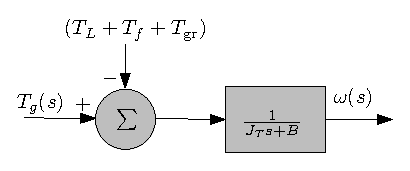
\includegraphics[width=0.4\textwidth]{figs/ipe/dcMotorMech}}
    }  
\caption{Block diagram representations of~\subref{fig:dcMotorElectric} electrical model~\eqref{eq:Ias} and~\subref{fig:dcMotorMech} mechanical  model~\eqref{eq:mechanicalModel}.}
\end{figure}
%
The mechanical equation is written as: %
%
\begin{subequations}
  \label{eq:mechanicalModel}
 \begin{align} 
    \label{eq:motorMechanical0}
    J_T\frac{\mathrm{d}\omega(t)}{\mathrm{dt}} & = T_g - T_D-T_L-T_f-T_{\mathrm{gr}},~~\mathrm{with}\\
    \label{eq:Tg0}
   T_g(t) & = K_TI_a(t)~\mathrm{and}\\
   \label{eq:TD0}
   T_D(t) & = B\omega(t).
\end{align}  
\end{subequations}
%
Taking Laplace transformation of model~\eqref{eq:motorMechanical0} and using the expression of $T_D$ in~\eqref{eq:TD0} yield: %
%
\begin{align}
  \label{eq:ws}
  \omega(s) =   \frac{1}{J_Ts +B}\left[T_g(s) - \left[T_L(s) + T_f(s) +T_{\mathrm{gr}}(s)\right]\right].
\end{align}
%
Figure~\ref{fig:dcMotorMech} shows the block diagram representation of model~\eqref{eq:ws} of a DC motor. Note that the elecric model~\eqref{eq:motorElectrical} and the mechanical model~\eqref{eq:motorMechanical0} of a PM DC motor are coupled through rotational speed $\omega$ and the armature current $I_a.$ Therefore, the electrical equations~\eqref{eq:electricModel} and mechanical equations~\eqref{eq:mechanicalModel} can be combined to form an electromechanical model of a DC motor as: %
%
  \begin{align}
    \label{eq:elecmechMotor}
  \begin{bmatrix}
    \frac{\mathrm{d}I_a}{\mathrm{dt}}\\
    \frac{\mathrm{d}\omega}{\mathrm{dt}}
  \end{bmatrix}
  = 
  \begin{bmatrix}
    -\frac{R_a}{L_a}  & -\frac{K_E}{L_a}\\
    \frac{K_T}{J_T}  & -\frac{B}{J_T}
  \end{bmatrix}
  \begin{bmatrix}
    I_a\\
    \omega
  \end{bmatrix}
+
  \begin{bmatrix}
    \frac{1}{L_a}\\
    0
  \end{bmatrix}
  V_a
-
  \begin{bmatrix}
    0\\
    \frac{1}{J_T}
  \end{bmatrix}
(T_L+T_f+T_{\mathrm{gr}}).
\end{align}
%
The block diagram representartion of the electromechanical model~\eqref{eq:elecmechMotor} is shown in Figure~\ref{fig:dcMotorElecMech}. %
%
\begin{figure}
  \centering
    \fcolorbox{white}{gray!15}{
  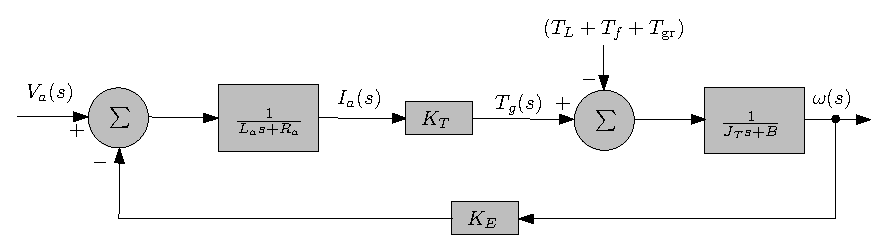
\includegraphics[width=0.6\textwidth]{figs/ipe/dcMotorElecMech}}
\caption{Block diagram representation of model~\eqref{eq:elecmechMotor}.}
\label{fig:dcMotorElecMech}
\end{figure}
%
Suppose that the motor is operating at no-load conditions and the friction torques are assumed to be negligible, \textit{i.e.,~}$T_L + T_f +T_{\mathrm{gr}} = 0,$ and the sum of mass moments of inertia of the motor $J_T$ is same as the motor's rotor inertia $J_m$ (\textit{i.e.,} $J_T=J_m).$ Then, the mechanical equation for  a permanent magnet brushed DC motor is simply
%
  \begin{align}
    \label{eq:motorMechanical}
    J_m\frac{\mathrm{d}\omega(t)}{\mathrm{dt}} = T_g - B\omega(t),
\end{align}  
%
which yields the motor transfer function given by: %
%
\begin{align}
  \label{eq:GM}
    G_M(s) = \frac{\omega(s)}{V_a(s)} = \frac{K_T}{\left(L_as + R_a\right)\left(J_Ts + B\right) + K_TK_E}.
\end{align}
%
Therefore, the electrical and mechanical time constants are %
%
\begin{align}
  \label{eq:timeConstants}
  \tau_E = \frac{L_a}{R_a}~\qquad\mathrm{and}~\qquad \tau_M = \frac{J_T}{B},
\end{align}
%
respectively. %
%
For simplicity, let us assume that the viscouse damping coefficient $B\approx 0$ and the armature inductance $L_a$ is very small (which is the case for most practical motors) compared to $R_a,$ the transfer function of a DC motor can be simplified as: %
%
\begin{align}
  G_m(s) = \frac{\omega(s)}{V_a(s)} = \frac{1/K_E}{(\tau_ms+1)(\tau_es+1)},
  \label{eq:motorTF}
\end{align}
%
where $\tau_m = \frac{R_aJ_T}{K_EK_T}$ and $\tau_e = \frac{L_a}{R_a}$ are the simplified mechanical and electrical time constants of the motor.

\section{Transient Response of Brushed DC Motor}
\label{sec:motorShaftspeedTransient}
This section illustrates the transient behavior of a PM brushed DC motor. For that, the rotor speed of a motor is determined as a function time for an applied voltage $V_a$ across its armature terminals. Clearly, the motor the simplified motor transfer function~\eqref{eq:motorTF} can be written as: %
%
\begin{align}
  \omega(s) = \frac{\left(1/K_E\right)V_a(s)}{(\tau_ms+1)(\tau_es+1)}.
  \label{eq:wSimplified}
\end{align}
%
Suppose that the applied voltage $V_a(t)$ to the motor terminals is constant (\textit{i.e.,} $V_a(t) = V_a).$ Taking the inverse Laplace transformation of $\omega(s),$ $\mathscr{L}^{-1}[\omega(s)]$ and using~\eqref{eq:wSimplified}  give the rotational speed of the rotor (armature)  expressed by: %
%
\begin{align}
  \omega(t) = \frac{V_a}{K_E}\left[1 + \frac{\tau_m}{\tau_e-\tau_m}e^{-t/\tau_m}+\frac{\tau_e}{\tau_m-\tau_e}e^{-t/\tau_e}\right].
  \label{eq:motorSpeedSO}
\end{align}
%
%
Note that the speed computed by Equation~\eqref{eq:motorSpeedSO} is in~[\si{\radian\per\second}]. The relationship between the motor speed in~[\si{\radian\per\second}] and that in revolutions per minute (RPM) is given by %
%
\begin{align}
  \omega(t) = \omega_{\mathrm{rpm}}(t) \times \frac{2\pi}{60},
  \label{eq:speedConversion}
\end{align}
%
where $\omega_{\mathrm{rpm}}(t)$ is the motor's rotational speed in~[rpm] at time $t\ge 0.$ If the gear ratio of the motor is $N:1,$ then the actual motor speed (motor's shaft speed) is computed using: %
%
\begin{align}
  \omega_{\mathrm{rpm,shaft}}(t) = \frac{\omega_{\mathrm{rpm}}(t)}{N},
  \label{eq:shaftSpeed}
\end{align}
%
where $\omega_{\mathrm{rpm,shaft}}(t)$ is the motor's shaft speed in [rpm]. 
%  
% If the armature inductance is very small, then the motor transfer function~\eqref{eq:motorTF} reduces to %
% %
% \begin{align}
%   G_m(s) = \frac{\omega(s)}{V_a(s)} = \frac{1/K_E}{\tau_ms+1},
%   \label{eq:motorTF-FirstOrder}
% \end{align}
% %
% In that case, the speed of the motor (in time domain) for an applied voltage of $V_a$ is given by %
% %
% \begin{align}
%   \omega(t) = \frac{V_a}{K_E}\left[1-e^{-t/\tau_m}\right].
%   \label{eq:motorSpeedFO}
% \end{align}
% %
%

\section{Steady-state Operating Conditions}
\label{sec:steadyStateOperatingConditions}
The no-load speed, $\omega_0,$ the no-load armature current, $I_0,$ and the motor's back-emf constant can be computed from the steady-state conditions (\textit{i.e.,} at time $t\to\infty$). Note that the load torque $T_L=0$ when the motor operates at no-load condition. At steady-state, the motor shaft speed is constant. Therefore, the steady-state speeds are denoted as: $\omega(t) =  \omega_0,~\omega_{\mathrm{rpm}}(t) =  \omega_{0,\mathrm{rpm}}, $ and $\omega_{\mathrm{shaft}}(t) =  \omega_{0,\mathrm{shaft}}.$  In addition, at steady-state,  $\frac{\mathrm{d}\omega(t)}{dt} = 0,$  $\frac{\mathrm{d}I_a(t)}{\mathrm{dt}} = 0,$ and $I_a = I_0.$  Therefore,  the mechanical Equation~\eqref{eq:motorMechanical} of the motor can be written as: $0 = T_g(t) - B\omega_0 = K_TI_0 - B\omega_0.$ Therefore, the expression for the no-load current is simply: %
%
\begin{align}
  I_0 = \frac{B\omega_0}{K_T}.
  \label{eq:noLoadCurrent}
\end{align}
%
Under steady-state operating conditions, the motor's electrical Equation~\eqref{eq:motorElectrical} can be rewritten as: %
%
\begin{align}
  V_a(t)= I_0R_a + V_b(t) = I_0R_a + K_E\omega_0.
  \label{eq:steadyStateElectricalEquation}
\end{align}
%
Suppose that the motor's applied voltage $V_a(t) = V_a$ is constant. Substituting the expression for the motor's no-load current in Equation~\eqref{eq:steadyStateElectricalEquation} yields the expression for the motor's no-load speed as: %
%
\begin{align}
  \omega_0 = \frac{V_a}{\frac{BR_a}{K_T} + K_E}.
  \label{eq:noLoadSpeed}
\end{align}
%
The expression for the motor's back-emf constant is given by:
\begin{align}
  K_E = \frac{V_a- I_oR_a}{\omega_0}.
  \label{eq:motorBackEmfConstant}
\end{align}
%
The viscous damping coefficient, $B,$ can also be computed from the steady-state operating condition of a DC motor. Suppose that the motor's applied voltage to its armature terminals gives a  no-load speed of $\omega_0~[\si{\radian\per\second}].$ Then the viscous damping coefficient %
%
\begin{align}
  B= \frac{K_T}{R_a}\left[\frac{V_a}{\omega_0} - K_E\right]. 
\end{align}
%
If the no-load motor shaft speed is given in [rpm], the rotor speed of the motor (\textit{i.e.,} motor's internal rotor speed), $\omega_0,$ is related to the motor shaft speed as: %
%
\begin{align}
  \omega_0 = N\times \omega_{0,\mathrm{shaft}}\times \frac{2\pi}{60}.
  \label{eq:speedConversion1}
\end{align}
%

\section{Measuring Steady-State Shaft Speed}
\label{sec:measuringShaftSpeed}
To measure the motor's internal speed, channel~$\#1$ (or channel~$\#2$) of the optical rotary encoder can be connected to an oscilloscope channel to graphically display the pulses produced by the encoder while the motor is rotating with an input voltage applied to its terminals. Since the rotary encoder has a resolution of $500$ pulses per revolution, the motor's internal speed is related to the encoder's frequency of the pulses by:
%
\begin{align}
  f_{\mathrm{encoder}} = \left(\frac{500}{60}\right)\omega_{0,\mathrm{rpm}},
  \label{eq:frequencyEncoder}
\end{align}
%
where $f_{\mathrm{encoder}}$ is the frequency of the encoder's output channel (channel~$\#1$ or channel~$\#2$) and  $\omega_{0,\mathrm{rpm}}$ is the motor's internal speed at steady state. Given the motor's encoder frequency, the motor's shaft speed can be computed using %
%
\begin{align}
  \omega_{0,\mathrm{shaft}} = \frac{1}{N}\left(\frac{60}{500}\right)f_{\mathrm{encoder}}.
  \label{eq:shaftSpeedMeasured}
\end{align}
%


\section{Prelab}
\label{sec:prelabDC-MotorModeling}
Before you start working on the prelab, it is important to read the theoretical background of a permanent magnet DC motor discussed in section~\ref{sec:introduction}. Furthermore, the values of the motor parameters should be recorded from the datasheet of the Pittman DC motor\footnote{See the Pittman DC motor datasheet at \href{http://www.precisionmotorworks.com/pdf/Pittman_GM87xx.web.pdf}{http://www.precisionmotorworks.com/pdf/Pittman\_GM87xx.web.pdf} [Note: highlighted values in the datesheet may not correspond to the motor that is used in this laboratory experiment. Therefore, choose the correct values of the DC motor used for this laboratory experiment]}. %The datasheet of the DC motor used in this experiment can be found at %
%
% \url{http://www.precisionmotorworks.com/pdf/Pittman_GM87xx.web.pdf} %or %
% %
% \url{http://ee.bradley.edu/projects/proj2003/cntrlwrk/gm9000_pittman.pdf}
% %
%
\begin{prelab}[DC motor modeling using Simulink]{prelab:DC-MotorModelingSimulink}
As mentioned, this laboratory experiment deals with a permanent magnet brushed DC motor (see its schematic diagram shown in Figure~\ref{fig:DC-MotorSchematic}). Therefore, the motor's field intensity is fixed. 
%
\begin{enumerate}
\item Record the values of parameters from the motor's datasheet in the table below.

  \begin{center}
    \begin{tabular}{c|l|l|l}
      \toprule
      Symbol & Description & Value & Unit\\
      \toprule
      $B$&Viscous damping coefficient&$\ldots$&$[\si{\newton\cdot\meter\per(\radian\per\second)}]$\\
      $J_m$&Motor shaft's moment of inertia&$\ldots$&$[\si{\kilogram\meter}^2]$\\      
      $K_E$&Back-emf constant &$\ldots$&$[\si{\volt\per(\radian\per\second)}]$\\
      $K_T$&Motor torque constant &$\ldots$&$[\si{\newton\meter\per\ampere}]$\\
      $L_a$&Armature inductance &$\ldots$&$[\si{\henry}]$\\            
      $R_a$&Armature resistance &$\ldots$&$[\si{\ohm}]$\\
      $N:1$&Gear reduction ratio &$\ldots$&N/A\\      
      \bottomrule
    \end{tabular}    
  \end{center}
\item Determine the values of the electrical $(\tau_E)$ and mechanical $(\tau_M)$ time constants.
%
  \begin{center}
    \begin{tabular}{c|c|c}
      \toprule
      Time constant &  Computed & Datasheet value\\
      \toprule
      $\tau_E$ & $\ldots$ & $\ldots$\\
      $\tau_M$ & $\ldots$ & $\ldots$\\
      \bottomrule
    \end{tabular}    
  \end{center}
\item  ~[Linear model] Use Simulink to model the brushed DC motor represented by the block diagram shown in Figure~\ref{fig:dcMotorElecMech}, where the motor is operating at no-load conditions and the friction torques are assumed to be negligible, \textit{i.e.,~}$T_L + T_f +T_{\mathrm{gr}} = 0,$ and the sum of mass moments of inertia of the motor $J_T$ is same as the motor's rotor inertia $J_m$ (\textit{i.e.,} $J_T=J_m).$
\item Run the Simulink model constructed in the previous step for $0.4~[\second]$, record the motor's no-load shaft speed and its no-load current (at steady state) for different applied voltages $V_a,$ and then complete the Table below: %
  %
%
  \begin{center}
    \begin{tabular}{c|c|c|c|c}
      \toprule
      $V_a~[\volt]$ &$\omega_{0,\mathrm{shaft,rpm}}$ (datasheet) &  $\omega_{0,\mathrm{shaft,rpm}}$ & $I_0~[\milli\ampere]$ & $f_{\mathrm{encoder}}$\\
      \toprule
      $0$ & $\ldots$ & $\ldots$& $\ldots$ & $\ldots$\\
      $4$ & $\ldots$ & $\ldots$& $\ldots$ & $\ldots$\\
      $8$ & $\ldots$ & $\ldots$& $\ldots$ & $\ldots$\\
      $12$ & $\ldots$ & $\ldots$& $\ldots$ & $\ldots$\\
      $16$ & $\ldots$ & $\ldots$& $\ldots$ & $\ldots$\\
      $20$ & $\ldots$ & $\ldots$& $\ldots$ & $\ldots$\\
      $24$ & $\ldots$ & $\ldots$& $\ldots$ & $\ldots$\\
      \bottomrule
    \end{tabular}    
  \end{center}  
  %
  Note that the no-load speed from the motor specification datasheet is computed using %
  %
  \begin{align}
    \omega_{0,\mathrm{shaft,rpm}}~~\mathrm{(datasheet)} = \left(\frac{\omega_{0,\mathrm{shaft,rpm}}^{\mathrm{max}}}{V_a^{\mathrm{ref}}}\right)V_a,
  \end{align}
  %
  where $\omega_{0,\mathrm{shaft,rpm}}^{\mathrm{max}}$ is the maximum RPM speed (shaft) of the motor at its reference voltage $V_a^{\mathrm{ref}}.$ 

\item ~[Nonlinear model] Use Simulink to model the brushed DC motor represented by the block diagram shown in Figure~\ref{fig:dcMotorElecMech}, where the motor is operating at no-load conditions in the presence of friction torque, \textit{i.e.,~}$T_L + T_f +T_{\mathrm{gr}} = T_f\ne 0,$ and the sum of mass moments of inertia of the motor $J_T$ is same as the motor's rotor inertia $J_m$ (\textit{i.e.,} $J_T=J_m).$ Note that $T_g-T_f\in[0,1000]~\si{\newton\meter},$ which adds the  nonlinearity to the DC motor simulink model. [Hint: add a saturation block before the block representing the mechanical transfer function shown in Figure~\ref{fig:dcMotorElecMech}.]
  
\item Run the Simulink model constructed in the previous step for $0.4~[\second]$, record the motor's no-load shaft speed and its no-load current (at steady state) for different applied voltages $V_a,$ and then complete the Table below: %
  %
%
  \begin{center}
    \begin{tabular}{c|c|c|c|c}
      \toprule
      $V_a~[\volt]$ &$\omega_{0,\mathrm{shaft,rpm}}$ (datasheet) &  $\omega_{0,\mathrm{shaft,rpm}}$ & $I_0~[\milli\ampere]$ & $f_{\mathrm{encoder}}$\\
      \toprule
      $0$ & $\ldots$ & $\ldots$& $\ldots$ & $\ldots$\\
      $4$ & $\ldots$ & $\ldots$& $\ldots$ & $\ldots$\\
      $8$ & $\ldots$ & $\ldots$& $\ldots$ & $\ldots$\\
      $12$ & $\ldots$ & $\ldots$& $\ldots$ & $\ldots$\\
      $16$ & $\ldots$ & $\ldots$& $\ldots$ & $\ldots$\\
      $20$ & $\ldots$ & $\ldots$& $\ldots$ & $\ldots$\\
      $24$ & $\ldots$ & $\ldots$& $\ldots$ & $\ldots$\\
      \bottomrule
    \end{tabular}    
  \end{center}  
  %
\end{enumerate}

\end{prelab}
%
% Before pursuing the next prelab, refer to section~\ref{sec:motorShaftspeedTransient} to see how the transient behavior of a PM blushed DC motor is modeled.  
\begin{prelab}[DC motor transient response]
~  
  %Attention is shifted to determine the motor speed as a function of time under no-load conditions with negligible frictions. %
  \begin{enumerate}
\item  Using the motor parameters recorded earlier, find the transfer function, $G_m(s) = \frac{\omega(s)}{V_a(s)},$ in complex frequency (Laplace) domain. [{\it Hint: Use Equation~\eqref{eq:motorTF}}].    
\item In one plot, show the motor speeds $\omega(t)$ (in [rpm]) versus time $t$ for the motor's applied voltages $V_a=0~[\volt],$ $4~[\volt],$ $8~[\volt],$ $12~[\volt],$ $16~[\volt],$ $20~[\volt],$ and $24~[\volt]$ using MATLAB.  [{\it Hint: Compute motor speeds using Equation~\eqref{eq:motorSpeedSO} for $t=0,~0.0001,~0.0002,\ldots, 0.25~[\second]$ for each applied voltage $V_a,$ then use Equations~\eqref{eq:speedConversion}~and~\eqref{eq:shaftSpeed}.}]

\item Record motor no-load shaft speeds and its no-load currents  for each applied voltage $V_a$ as in Table below: %
%
  \begin{center}
    \begin{tabular}{c|c|c}
      \toprule
      $V_a~[\volt]$ &  $\omega_{0,\mathrm{shaft}}$~[rpm] & $I_0~[\milli\ampere]$\\
      \toprule
      $0$ & $\ldots$ & $\ldots$\\
      $4$ & $\ldots$ & $\ldots$\\
      $8$ & $\ldots$ & $\ldots$\\
      $12$ & $\ldots$ & $\ldots$\\
      $16$ & $\ldots$ & $\ldots$\\
      $20$ & $\ldots$ & $\ldots$\\
      $24$ & $\ldots$ & $\ldots$\\
      \bottomrule
    \end{tabular}    
  \end{center}
%
[\emph{Hint:To compute no-load shaft speed, use Equation~\eqref{eq:noLoadSpeed} followed by the speed conversion Equation~\eqref{eq:speedConversion1} and use Equation~\eqref{eq:noLoadCurrent}  to compute the no-load armature current.}]
\end{enumerate}
\end{prelab}




\section{Laboratory Work}
Two power supplies are required to conduct this experiment. The first power supply ({\bf Agilent E3630} $\mathbf{0}$-$\mathbf{6}~[\volt],$ $\pm 20~[\volt]$ power supply which is already available at the workstation) is needed to turn on the rotary encoder (used for measuring rotational speed) of the motor. The second power supply ($30$V HP 6215 supply) is used for the motor's applied voltage (armature voltage) at the \emph{Motor + - terminals}.

\begin{mdframed}
  {\bf NOTE: HAVE YOUR INSTRUCTOR OR A TEACHING ASSISTANT CHECK YOUR MOTOR CIRCUIT BEFORE TURNING IT ON.}  
\end{mdframed}

\begin{enumerate}
\item Connect the encoder circuit as shown in Figure~\ref{fig:pittmanDC-MotorKit}. 
\item Use the Agilent E3630 $\mathbf{0}$-$\mathbf{6}~[\volt]$ option  as the voltage source $V_E$ to supply $V_E = 5.7~[\volt]$ to the rotary encoder of the motor.
\item Connect channel~1 (or channel~2) of the rotary encoder mounted on the DC motor's kit to channel~1 of the oscilloscope at your workstation. 
\item Use $30$V HP 6215  power supply to supply $V_a=4~[\volt]$ to the Motor \emph{+/-} terminals and record the speed by observing the pulse waveform on the oscilloscope. Note that the rotary encoder produces $500$ pulses per revolution. Repeat for $V_a=8~[\volt],~\ldots,~24~[\volt]$ and record the measured motor speed in the table below: %
%
  \begin{center}
    \begin{tabular}{c|c|c|c}
      \toprule
      $V_a~[\volt]$ &  $\omega_{0,\mathrm{shaft, rpm}}$ (measured)&  $\omega_{0,\mathrm{shaft,rpm}}$ (computed) & Error (\%)\\
      \toprule
      $0$ & $\ldots$ & $\ldots$& $\ldots$\\
      $4$ & $\ldots$ & $\ldots$& $\ldots$ \\
      $8$ & $\ldots$ & $\ldots$& $\ldots$ \\
      $12$ & $\ldots$ & $\ldots$& $\ldots$ \\
      $16$ & $\ldots$ & $\ldots$& $\ldots$ \\
      $20$ & $\ldots$ & $\ldots$& $\ldots$ \\
      $24$ & $\ldots$ & $\ldots$& $\ldots$ \\
      \bottomrule
    \end{tabular}    
  \end{center}

\item Connect the ammeter in series with the armature circuit of the motor as shown in Figure~\ref{fig:DC-MotorSchematicMeasuringNoLoadCurrent} and measure the no-load current for the motor's applied voltage $V_a=0,~4~[\volt],~8~[\volt],~\ldots,~24~[\volt].$ %
%
  %
\begin{figure}
  \centering
    \begin{circuitikz}[scale=1.2,american voltages]
      \draw
      (-3*\smgrid,0) to[short,o-](8*\smgrid,0) to[Telmech=M,n=motor,fill=red!50] (8*\smgrid,4*\smgrid);
      \draw[thick,->>]
      (motor.right) -- (10*\smgrid,2*\smgrid)node[midway,above]{$\omega$};
      \draw
      (-3*\smgrid,4*\smgrid) to[ammeter,v>=~,o-,l^=$I_0$,fill=yellow!50]
      (0,4*\smgrid) to[R,l^=$R_a$,i>=~] (4*\smgrid,4*\smgrid) to [cute inductor,l^=$L_a$](8*\smgrid,4*\smgrid);
      \draw
      (-3.5*\smgrid,0) to[open,v<=$V_a$] (-3.5*\smgrid,4*\smgrid);
      \node at(7*\smgrid,2*\smgrid){$V_b$};
      \node at(7*\smgrid,3*\smgrid){$+$};
      \node at(7*\smgrid,1*\smgrid){$-$};

    \end{circuitikz}
    
    \caption{DC motor schematic diagram for measuring no-load current $I_0.$}
    \label{fig:DC-MotorSchematicMeasuringNoLoadCurrent}    
\end{figure}
%
Record the measured no-load current in the table below: %
%
  \begin{center}
    \begin{tabular}{c|c|c|c}
      \toprule
      $V_a~[\volt]$ &  $I_0$ (measured) ~[\milli\ampere]&  $I_0$ (computed) ~[\milli\ampere] & Error (\%)\\
      \toprule
      $0$ & $\ldots$ & $\ldots$& $\ldots$\\
      $4$ & $\ldots$ & $\ldots$& $\ldots$ \\
      $8$ & $\ldots$ & $\ldots$& $\ldots$ \\
      $12$ & $\ldots$ & $\ldots$& $\ldots$ \\
      $16$ & $\ldots$ & $\ldots$& $\ldots$ \\
      $20$ & $\ldots$ & $\ldots$& $\ldots$ \\
      $24$ & $\ldots$ & $\ldots$& $\ldots$ \\
      \bottomrule
    \end{tabular}    
  \end{center}  



\item Comment on any discrepancy found between the computed and the experimental (measured) values of the no-load speeds  and and no-load currents. 
\end{enumerate}


%%% Local Variables:
%%% mode: latex
%%% TeX-master: "../../labBookMechatronics-V2"
%%% End:
